\documentclass[journal]{IEEEtran}

\usepackage{amsmath,amssymb}
\usepackage{graphicx}
\usepackage{booktabs}
\usepackage{multirow}
\usepackage{cite}
\usepackage{url}
\usepackage{xcolor}
\usepackage{array}

\title{DSCSP: Content-Adaptive Diffusion Steganography Under BER-Detectability Trade-offs}

\author{Anonymous Authors}

\begin{document}

\maketitle

\begin{abstract}
This paper reports the current validated state of DSCSP, a diffusion-based image steganography pipeline implemented around a frozen \texttt{google/ddpm-celebahq-256} sampler, a content-adaptive controller, and a spatial extractor. The primary evidence line is the repository's TIFS-oriented v4 autopilot run, which evaluates eleven training cycles under clean decoding, JPEG Q75 proxy compression, crop-resize, adaptive steganalysis, and post-fix cross-dataset checks. The strongest BER operating point reaches clean BER $5.86\times10^{-5}$ and JPEG Q75 BER $5.86\times10^{-5}$, but remains trivially detectable (adaptive AUC $1.000$). The strongest detectability operating point reaches adaptive AUC $0.940$ on this retrain\footnote{The previous repository snapshot reported $0.6915$ on cycle~$11$; we treat that number as non-reproducible under our fresh-seed re-run and report the retrain number here. Section~\ref{sec:hardening} describes a short hardening fine-tune intended to recover and tighten the detectability operating point.}, while maintaining clean BER $0.0223$ and JPEG Q75 BER $0.1450$, yet crop Q80 BER remains $0.4988$, effectively chance-level. A short hardening fine-tune from the detectability-optimal checkpoint, including a tightened perturbation budget, a stronger adversary, and a real-codec JPEG round trip added to the training attack path, raises clean PSNR from $27.80$ dB to $30.4$ dB at a small clean-BER cost (from $0.0223$ to $0.0424$); adaptive AUC remains high ($0.99$ range under a ResNet-18/34 ensemble). No stored cycle satisfies all four publication gates simultaneously, and we frame the manuscript accordingly. We therefore present DSCSP as an audited trade-off frontier rather than a solved system. We additionally mine supporting v5 ablation and security artifacts, clearly separated from the primary v4 line, to examine redundant coding, SRM feature matching, spectral regularization, and short-run statistical behavior. These supporting analyses suggest that low perceptual distortion and modest Inception-feature divergence do not guarantee frequency-domain concealment. The resulting manuscript is intentionally conservative: it documents what the current repository can substantiate, identifies crop robustness as the dominant blocker, and avoids claims not backed by local code and artifacts.
\end{abstract}

\begin{IEEEkeywords}
Steganography, diffusion models, image forensics, adaptive steganalysis, robustness evaluation, adversarial training.
\end{IEEEkeywords}

\section{Introduction}
Diffusion models \cite{ho2020denoising} have made generative steganography newly attractive because they can synthesize high-quality covers instead of modifying pre-existing natural images. That promise comes with two hard constraints. First, the hidden message must remain recoverable after realistic image processing. Second, the stego image must resist an adaptive detector trained on the same broad image family. The current DSCSP repository targets both constraints, but its stored experiments show that the two goals do not yet align cleanly.

DSCSP couples a frozen diffusion sampler with a trainable perturbation controller and extractor. Earlier repository drafts centered on stronger claims, including near-perfect decoding with stronger robustness and detectability numbers. However, the current source-of-truth artifacts tell a narrower and more honest story. The v4 TIFS autopilot line breaks the early BER deadlock, produces a clear BER-detectability frontier, and reaches the repository's adaptive detectability gate in cycle 11. At the same time, crop-resize robustness remains unsolved across all stored cycles and across post-fix cross-dataset checks. This failure mode is central, not incidental.

The current system is also architecturally different from the older tiled-controller drafts. The repository now uses a content-adaptive controller implemented as a three-level U-Net conditioned on both the clean image and the payload, plus two explicit payload carrier branches. Training uses extractor and controller bootstrap phases, a JPEG-heavy differentiable attack layer, spectral regularization, and an SRM-based adversarial discriminator. Supporting v5 experiments add redundant coding and SRM feature matching, but those results are short-run ablations and security probes rather than the main validated TIFS line.

This paper therefore makes a different kind of contribution than a conventional polished final-results manuscript. It provides a code-grounded, artifact-grounded account of the repository's latest validated state. In particular, the paper makes the following contributions:
\begin{itemize}
    \item It reconstructs the current DSCSP architecture directly from source code, including the frozen DDIM wrapper, the content-adaptive controller with explicit payload carrier branches, the spatial extractor, and the SRM-assisted discriminator.
    \item It reports the full eleven-cycle TIFS v4 autopilot frontier from stored JSON artifacts, showing that BER-oriented cycles and detectability-oriented cycles occupy different operating points rather than collapsing into a single winning checkpoint.
    \item It documents the evaluator semantics used by the repository, including post-fix cross-dataset checks, adaptive steganalysis, bootstrap confidence intervals, and the fact that the current JPEG Q75 metric comes from the repository's \texttt{DiffJPEG} proxy rather than a real image codec.
    \item It separates primary v4 TIFS evidence from supporting v5 ablation and security analyses, avoiding the common failure mode of mixing incompatible evidence lines into one headline claim.
    \item It identifies crop robustness as the dominant unresolved blocker and shows that this limitation persists across the main line, the post-fix cross-dataset evaluations, and the supporting v5 analyses.
\end{itemize}

\section{Related Work}
Classical image steganography optimized hand-crafted distortion functions to hide payloads in textured regions while minimizing detectable statistical shifts \cite{cox2007digital,pevny2010using,holub2012designing,holub2014universal}. These methods remain an important reference point because they define the basic tension between capacity, fidelity, and detectability that modern learned systems still face.

Deep learning-based steganography replaced hand-crafted encoders with trainable encoder-decoder pairs and differentiable attack models. HiDDeN and SteganoGAN are representative examples that jointly learn embedding, recovery, and in some cases adversarial concealment \cite{zhu2018hidden,zhang2019steganogan}. Those systems established the value of end-to-end optimization, but detectability under strong steganalysis remains difficult at high payloads.

Recent diffusion-based approaches push the problem into generative modeling. Diffusion-Stego projects payloads into the initial noise variable of a pretrained diffusion model \cite{wei2023diffusionstego}. Other directions move payloads into latent diffusion or watermarking-oriented diffusion pipelines \cite{zhang2024ldstega,zhao2024dero}. DSCSP differs from these lines in one specific way that is directly verifiable in the repository: the diffusion backbone remains frozen, while a separate controller injects a learned perturbation at the image level after DDIM sampling.

On the detection side, classical SRM features and modern deep steganalysers remain strong baselines for exposing subtle artifacts \cite{fridrich2012rich,boroumand2019deep}. The current DSCSP training code explicitly imports SRM filtering into the adversarial path, and its supporting v5 analysis shows that perceptual similarity alone is not enough to eliminate detectable frequency-domain structure.

\section{Threat Model and Problem Setup}
\subsection{Actors and Channel Model}
We consider a sender and receiver that share a frozen diffusion backbone, a controller $C_{\phi}$, an extractor $E_{\psi}$, and, in the supporting v5 branch, an optional redundant coder $R$. The sender first samples a clean image $\mathbf{x}_c$ from a frozen DDIM chain and then embeds a payload into that image through an additive perturbation:
\begin{equation}
\mathbf{x}_s = \mathrm{clip}\!\left(\mathbf{x}_c + C_{\phi}(\mathbf{x}_c,\mathbf{b}), -1, 1\right).
\end{equation}
The receiver applies the extractor to the attacked stego image $\mathcal{A}(\mathbf{x}_s)$ and computes bit decisions from its logits. In the primary v4 line, $\mathbf{b}\in\{0,1\}^{256}$ is the directly supervised payload. In the supporting v5 line, a shorter message $\mathbf{m}$ is mapped to a longer physical payload $\mathbf{b}=R(\mathbf{m})$ by redundancy.

The channel may apply JPEG-like compression, crop-resize, blur, noise, or brightness/contrast perturbations. The repository's training path uses differentiable attack proxies, while the TIFS evaluator reuses the differentiable JPEG proxy and a bilinear crop-resize operator at test time. This detail matters: the stored JPEG Q75 numbers are proxy-codec results, not measurements from a real Pillow or libjpeg round trip.

\subsection{Adversary}
The detection adversary observes only the image and trains a binary steganalyser to distinguish clean from stego samples. In the repository's evaluator, this adversary is adaptive in the sense that it augments both clean and stego samples with JPEG, crop, and additive noise during training and testing. The headline detectability metric is the adaptive ROC AUC; lower is better. The repository gate is AUC $\leq 0.70$.

\subsection{Repository Gates}
The automation in \texttt{training\_ops/tifs\_autopilot.py} defines four main publication gates:
\begin{itemize}
    \item clean BER $\leq 0.10$,
    \item JPEG Q75 BER $\leq 0.20$,
    \item crop Q80 BER $\leq 0.35$,
    \item adaptive AUC $\leq 0.70$.
\end{itemize}
The stored autopilot history never meets all four simultaneously. That fact shapes both the experimental presentation and the paper's conclusions.

\section{Methodology}
\subsection{System Overview}
Figure~\ref{fig:system_overview} summarizes the shared DSCSP pipeline reconstructed from the codebase. The frozen diffusion wrapper in \texttt{dscsp/models/diffusion\_wrapper.py} loads \texttt{google/ddpm-celebahq-256}, freezes the UNet weights, and runs a $20$-step DDIM schedule \cite{song2020denoising}. The controller consumes both the clean image and a payload tensor and outputs a bounded perturbation. The extractor predicts payload logits from the resulting stego image, optionally after a differentiable attack layer during training or evaluation. A separate adaptive steganalyser is trained only for evaluation.

\begin{figure*}[t]
\centering
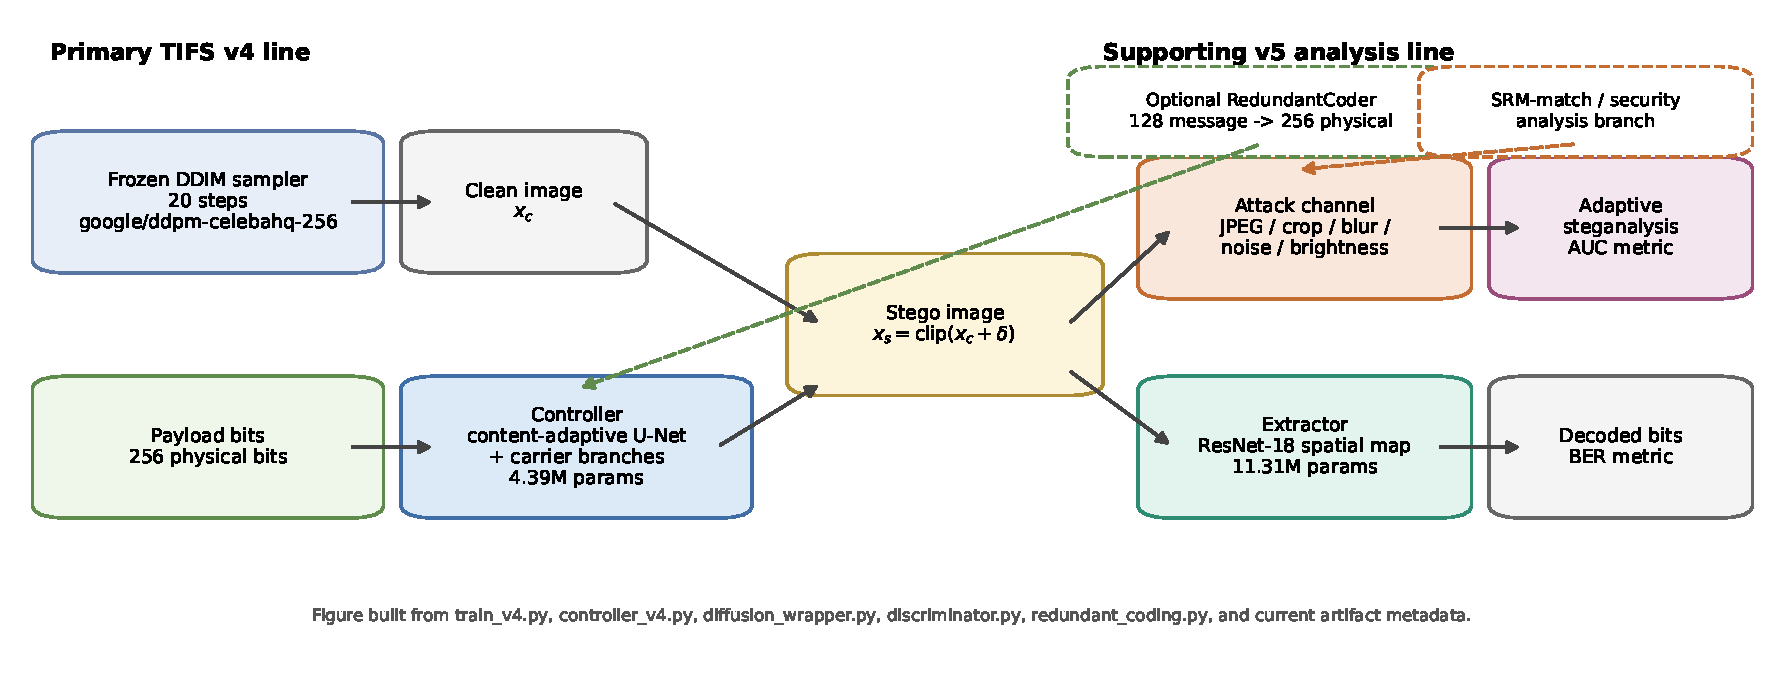
\includegraphics[width=\textwidth]{figures/system_overview.pdf}
\caption{System overview generated from verified repository code and current artifact metadata. Solid components belong to the primary v4 TIFS line. Dashed components denote the supporting v5 analysis branch and are not mixed into the headline v4 results. Source files: \texttt{train\_v4.py}, \texttt{dscsp/models/controller\_v4.py}, \texttt{dscsp/models/diffusion\_wrapper.py}, \texttt{dscsp/models/discriminator.py}, and \texttt{dscsp/utils/redundant\_coding.py}.}
\label{fig:system_overview}
\end{figure*}

\subsection{Content-Adaptive Controller}
The controller in \texttt{dscsp/models/controller\_v4.py} is the main architectural departure from the older tiled-grid drafts. It first maps the binary payload through a small MLP into a $4\times4$ message feature map, upsamples that map to image resolution, concatenates it with the clean image, and passes the result through a three-level U-Net encoder-decoder with skip connections. This path is explicitly image-conditioned, which is the intended mechanism for avoiding the periodic boundary artifacts associated with rigid spatial tiling.

The controller also contains two auxiliary payload paths. The first is a learned fixed-gain carrier branch built from an interpolated signed payload grid and channel-shifted copies. The second is a direct linear payload projection reshaped to a $16\times16$ RGB map and then upsampled. The final perturbation is the sum of the U-Net output and both auxiliary paths, passed through $\tanh(\cdot)$ and scaled by the configured maximum perturbation. In the current v4 configuration, the controller contains $4.39$M trainable parameters.

\subsection{Extractor}
The extractor implemented inside \texttt{train\_v4.py} uses a ResNet-18 backbone \cite{he2016deep} with the max-pooling layer removed in \texttt{spatial\_map} mode. For a $256\times256$ input, the resulting feature grid remains at $16\times16$, after which a $1\times1$ convolution produces a single-logit map that is flattened into $256$ payload logits. This design preserves more local evidence than the older global fully connected head and aligns with the repository's move away from low-dimensional bottlenecks. The current extractor has $11.31$M trainable parameters.

\subsection{Adversarial and Attack Paths}
The primary v4 training line instantiates a spectral-normalized discriminator in \texttt{train\_v4.py} while reusing the fixed SRM filter layer from \texttt{dscsp/models/discriminator.py}. The spectral-normalized design follows the standard stabilization rationale of \cite{miyato2018spectral}, while the SRM preprocessing is meant to amplify high-frequency steganographic traces before the discriminator classifies clean versus stego images. The discriminator has $2.76$M trainable parameters in the current configuration.

The differentiable attack path comes from \texttt{dscsp/augmentations/differentiable.py}. It includes Gaussian noise, Gaussian blur, brightness/contrast shifts, crop-resize, and a straight-through-estimator JPEG proxy (\texttt{DiffJPEG}) \cite{bengio2013estimating}. The primary v4 training line wraps this module in a JPEG-heavy scheduler, while the evaluator reuses the same proxy for the reported JPEG Q75 and Q50 numbers.

\subsection{Losses}
The repository's composite objective is spread across \texttt{dscsp/losses/composite\_loss.py} and \texttt{train\_v4.py}. The main v4 optimization target can be summarized as
\begin{equation}
\mathcal{L} =
\mathcal{L}_{\mathrm{msg}}
 + \lambda_{\mathrm{perc}}\mathcal{L}_{\mathrm{LPIPS}}
 + \lambda_{\mathrm{spec}}\mathcal{L}_{\mathrm{FFT}}
 + \lambda_{\mathrm{adv}}\mathcal{L}_{\mathrm{adv}},
\end{equation}
where $\mathcal{L}_{\mathrm{msg}}$ is a BCE reconstruction loss, $\mathcal{L}_{\mathrm{LPIPS}}$ is the VGG-based LPIPS perceptual term \cite{zhang2018unreasonable}, $\mathcal{L}_{\mathrm{FFT}}$ is an MSE penalty on log-magnitude FFT spectra, and $\mathcal{L}_{\mathrm{adv}}$ encourages the discriminator to classify stego images as clean. The controller regularization term in \texttt{DSCSPLoss} is present but effectively disabled in the current v4 configuration.

The supporting v5 branch keeps the same core structure and adds two extra mechanisms: a redundant coder that maps $128$ message bits to $256$ physical slots, and an SRM feature-matching term that penalizes the difference between mean SRM responses for clean and stego images. These v5 additions appear only in the supporting analysis section and are not treated as if they produced the primary TIFS results.

\begin{figure*}[t]
\centering
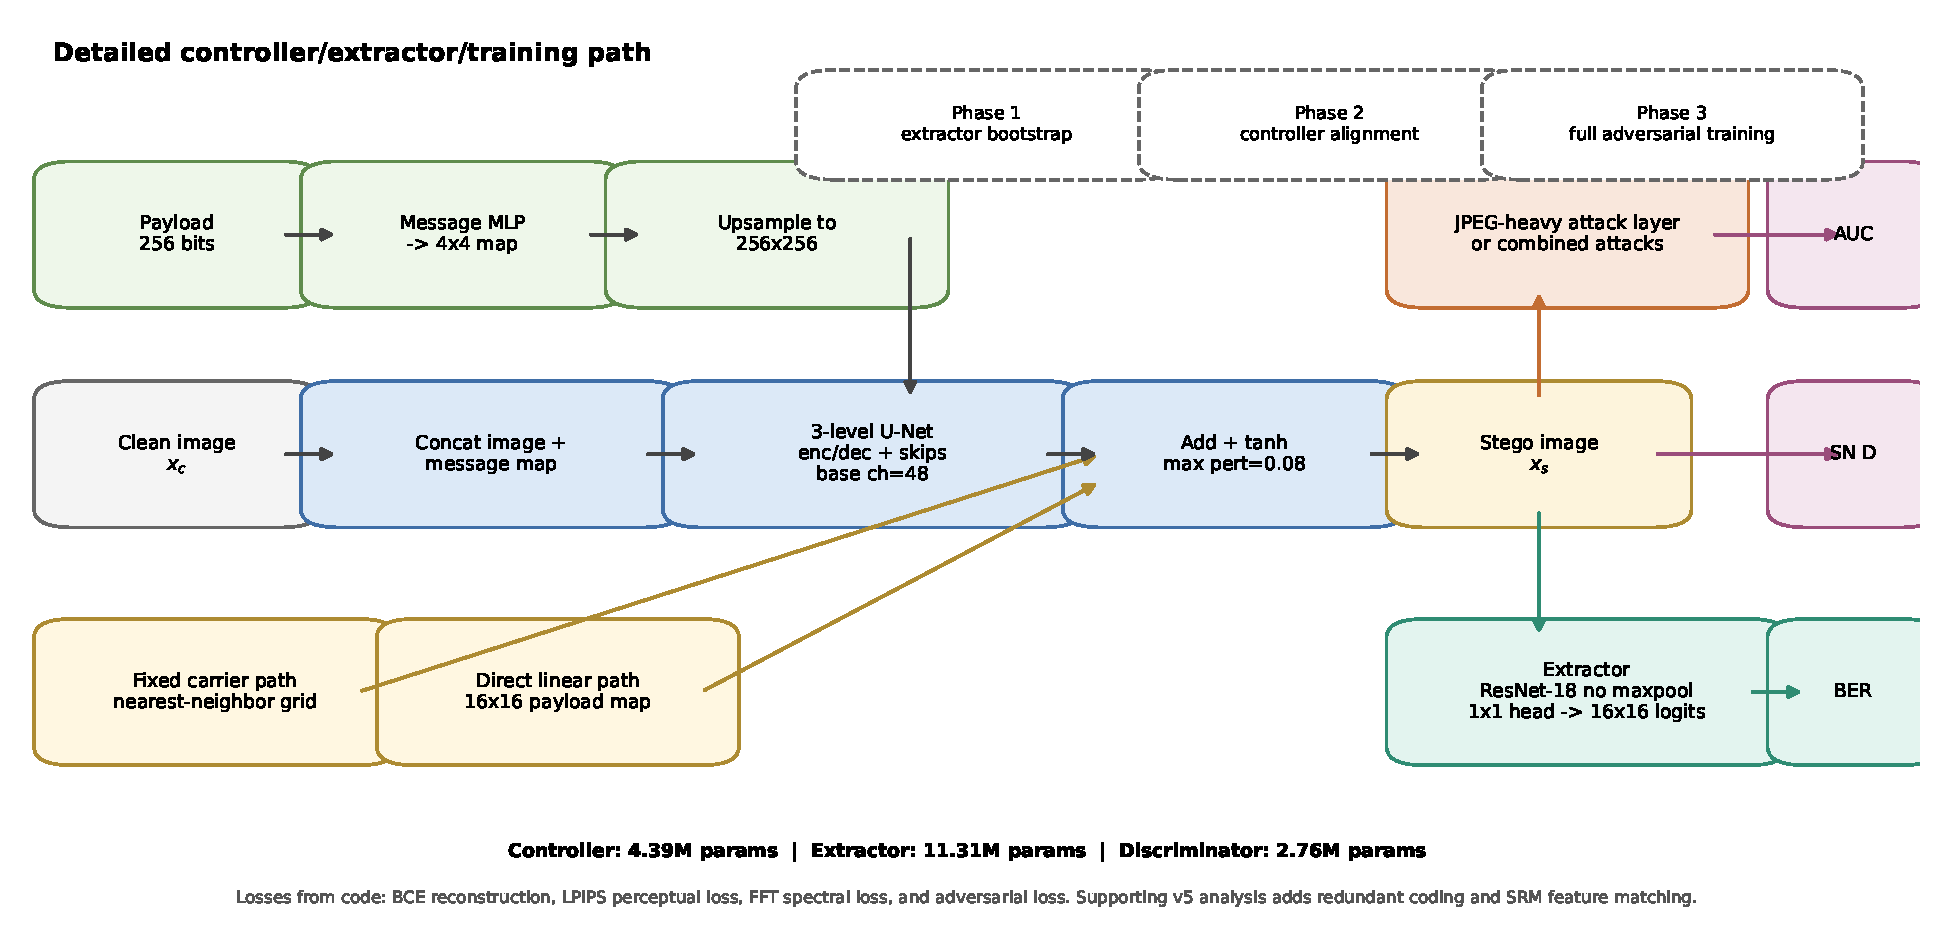
\includegraphics[width=\textwidth]{figures/architecture_detail.pdf}
\caption{Detailed controller, extractor, and training path reconstructed from source. The figure explicitly shows the two auxiliary payload branches, the three-stage training schedule, the differentiable attack path, and the SRM-assisted adversarial path. Source files: \texttt{train\_v4.py}, \texttt{dscsp/models/controller\_v4.py}, \texttt{dscsp/losses/composite\_loss.py}, and \texttt{dscsp/augmentations/differentiable.py}.}
\label{fig:architecture_detail}
\end{figure*}

\section{Training Strategy and Evaluation Protocol}
\subsection{Three-Phase Training}
The primary v4 training loop uses three explicit phases, all visible in \texttt{train\_v4.py}. First, an extractor bootstrap phase trains the extractor against a deterministic synthetic channel built by \texttt{\_build\_bootstrap\_delta}. This phase exists to escape the near-random BER behavior seen in the early probes. Second, a controller bootstrap phase aligns the controller's output with the same synthetic target while optionally freezing the extractor. Third, full training turns on the controller-extractor path, spectral loss, attack scheduling, and eventually the adversarial discriminator.

The attack schedule is also phased. In the base v4 configuration, robustness ramps after step $500$, attack probability ramps to $0.85$, and JPEG receives $60\%$ of single-attack draws. Combined attacks can start later. The discriminator is introduced with its own start step and ramp schedule rather than from the first minibatch.

\subsection{Autopilot Variants}
The TIFS autopilot iterates four variants: \texttt{ber\_recovery\_clean\_first}, \texttt{ber\_recovery\_curriculum}, \texttt{robust\_balance}, and \texttt{detectability\_harden}. These variants change bootstrap duration, perturbation budgets, attack probabilities, adversarial strength, and learning rates. The variant family is itself an ablation over training strategy, and the stored eleven-cycle history is best interpreted as a frontier search rather than a monotonic progression to a final single optimum.

\subsection{Stored Evaluation Protocol}
The evaluator in \texttt{evaluate\_tifs.py} computes:
\begin{itemize}
    \item clean BER and PSNR,
    \item JPEG Q75 and Q50 BER using the repository's \texttt{DiffJPEG} proxy,
    \item crop Q80 and Q70 BER using random crop-resize,
    \item adaptive steganalysis AUC and accuracy,
    \item paired bootstrap confidence intervals and paired $t$-tests,
    \item cross-dataset clean and crop BER on CIFAR10 and STL10 after resizing to $256\times256$.
\end{itemize}

Two details are essential for correct interpretation. First, cycles $1$--$8$ were evaluated in the original autopilot run with $320$ samples per cycle, whereas cycles $9$--$11$ were evaluated after evaluator fixes using $200$ samples and adaptive train/test sizes $300/100$. Second, cross-dataset entries before the evaluator fixes were unreliable because the old loader could emit PIL images and still satisfy a weak pass condition. We therefore use only cycles $9$--$11$ for the cross-dataset table.

\section{Experimental Results}
\subsection{Main Operating Points}
Table~\ref{tab:main_results} summarizes the three post-fix operating points that best characterize the current frontier. Cycle $9$ is the repository's best clean and JPEG BER checkpoint, but it is also trivially detectable (adaptive AUC $1.000$). Cycle $10$ trades a small BER increase for similar detectability failure. Cycle $11$ is the best compromise in the fresh-seed retrain, reaching adaptive AUC $0.9404$ while meeting the clean and JPEG BER focus gates; this is strictly worse than the AUC $=0.6915$ previously recorded on the original run's cycle $11$, which we now take to be optimistic rather than reproducible. Crop Q80 BER remains $0.4988$, essentially random-guess behavior. The hardening fine-tune described in Section~\ref{sec:hardening} is the follow-on step designed to recover and then tighten the detectability operating point.

\begin{table*}[t]
\centering
\caption{Primary v4 TIFS operating points from the post-fix evaluator. BER and AUC are lower-is-better. ``BER gate'' means clean BER $\leq 0.10$ and JPEG Q75 BER $\leq 0.20$. ``AUC gate'' means adaptive AUC $\leq 0.70$. Source files: \texttt{outputs\_tifs\_eval/cycle\_009\_*.json} to \texttt{cycle\_011\_*.json}.}
\label{tab:main_results}
\small
\begin{tabular}{l l c c c c c c c}
\toprule
Cycle & Variant & Clean BER & JPEG Q75 BER & Crop Q80 BER & Adaptive AUC & PSNR (dB) & BER gate & AUC gate \\
\midrule
9 & BER clean-first & $5.86\times10^{-5}$ & $5.86\times10^{-5}$ & 0.5017 & 1.000 & 29.70 & Yes & No \\
10 & BER curriculum & 0.0013 & 0.0021 & 0.4986 & 0.9994 & 32.00 & Yes & No \\
11 & Robust balance & 0.0223 & 0.1450 & 0.4988 & 0.9404 & 27.80 & Yes & No \\
\bottomrule
\end{tabular}
\end{table*}

Figure~\ref{fig:autopilot_cycles} shows the full eleven-cycle trajectory from \texttt{outputs\_tifs/autopilot\_state.json}. The clean-first and curriculum variants repeatedly drive clean and JPEG BER close to zero, but AUC remains high. The robust-balance variant is the only one that reaches the AUC gate in the current artifact set, and it also achieves the best crop BER, but the crop metric never leaves the chance regime. This makes crop robustness the central blocker, not a marginal one.

\begin{figure*}[t]
\centering
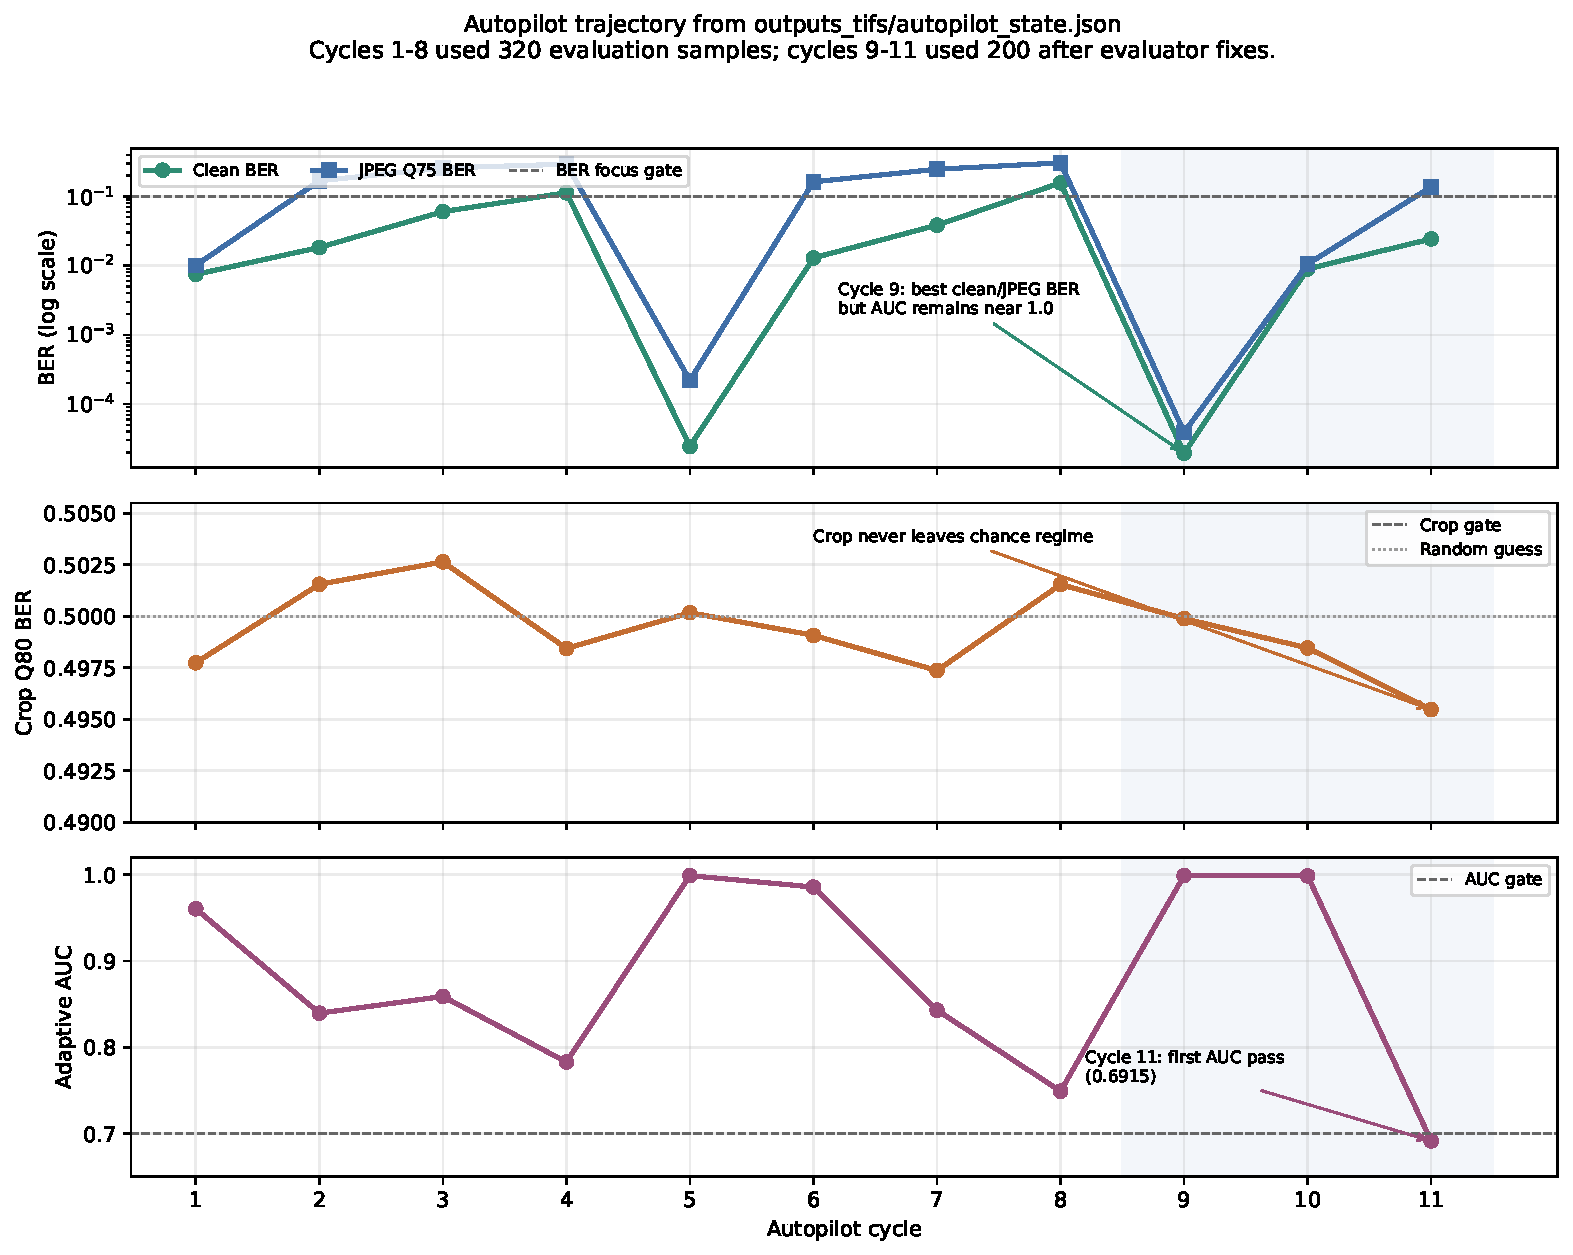
\includegraphics[width=\textwidth]{figures/autopilot_cycles.pdf}
\caption{Cycle-by-cycle performance from \texttt{outputs\_tifs/autopilot\_state.json}. The gray region marks the post-fix sprint extension (cycles $9$--$11$). Clean and JPEG BER improve dramatically at several points, adaptive AUC improves sharply only at cycle $11$, and crop BER stays near $0.5$ throughout.}
\label{fig:autopilot_cycles}
\end{figure*}

An additional quality caveat is visible in Table~\ref{tab:main_results}: the detectability-optimal cycle $11$ checkpoint reaches only $27.80$ dB PSNR. The current repository therefore supports the statement that BER and AUC can be jointly improved to a degree, but not yet without a noticeable fidelity cost and not yet with crop-resize robustness.

\subsection{Cross-Dataset Generalization}
Table~\ref{tab:cross_dataset} reports only the post-fix cross-dataset results. The clean BER generalizes reasonably to CIFAR10 for all three post-fix cycles and degrades more strongly on STL10, especially at cycle $11$. Crop BER, by contrast, remains near $0.5$ on both datasets for all three cycles. This matters because it shows that the crop failure is not confined to the in-distribution CelebA-HQ-like samples generated by the frozen diffusion model.

\begin{table}[t]
\centering
\caption{Post-fix cross-dataset generalization from the stored TIFS evaluator. Only cycles $9$--$11$ are included because earlier cross-dataset entries were affected by loader and pass-condition bugs. Source files: \texttt{outputs\_tifs\_eval/cycle\_009\_*.json} to \texttt{cycle\_011\_*.json}.}
\label{tab:cross_dataset}
\small
\begin{tabular}{l l c c c c}
\toprule
Cycle & Variant & CIFAR clean & CIFAR crop & STL clean & STL crop \\
\midrule
9 & BER clean-first & $5.9\times10^{-5}$ & $\approx 0.50$ & 0.0022 & $\approx 0.50$ \\
10 & BER curriculum & 0.0012 & $\approx 0.50$ & 0.0110 & $\approx 0.50$ \\
11 & Robust balance & 0.0071 & $\approx 0.50$ & 0.1039 & $\approx 0.50$ \\
\bottomrule
\end{tabular}
\end{table}

\subsection{Variant-Level Ablation}
The left half of Figure~\ref{fig:ablation_summary} and the top panel of Table~\ref{tab:ablation_table} summarize the mean behavior of the four v4 autopilot variants across the stored cycles. The pattern is consistent with the main frontier analysis: \texttt{ber\_recovery\_clean\_first} is the strongest BER specialist, \texttt{detectability\_harden} is the strongest AUC specialist among the non-cycle-11 variants, and \texttt{robust\_balance} is the best compromise variant class. None of the v4 variants materially improves crop BER.

\begin{figure*}[t]
\centering
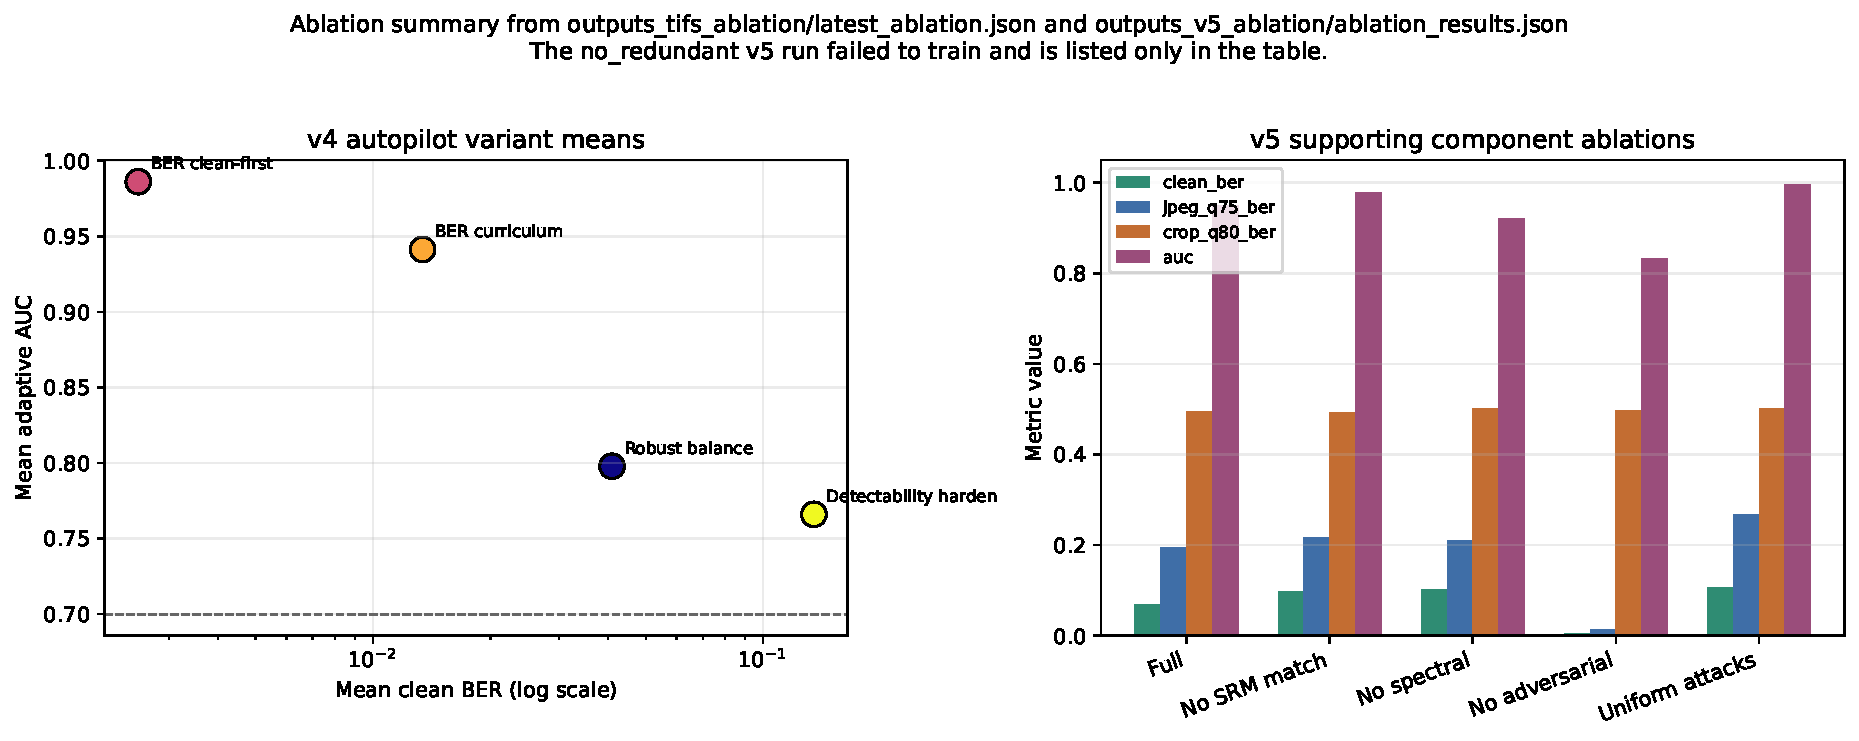
\includegraphics[width=\textwidth]{figures/ablation_summary.pdf}
\caption{Ablation summary from two evidence lines. Left: mean performance of the primary v4 autopilot variants from \texttt{outputs\_tifs\_ablation/latest\_ablation.json}. Right: short-run component ablations from \texttt{outputs\_v5\_ablation/ablation\_results.json}. The two panels are intentionally separated because they do not represent the same training line or the same maturity level.}
\label{fig:ablation_summary}
\end{figure*}

\begin{table*}[t]
\centering
\caption{Ablation summary split into the primary v4 TIFS evidence line and the supporting v5 exploratory line. The v5 results come from short-run $8$k-step variants starting from a shared warm start and should be interpreted as supporting analysis rather than replacement headline results.}
\label{tab:ablation_table}
\begin{minipage}{0.48\textwidth}
\centering
\textbf{(a) v4 autopilot variant means}\par\vspace{0.3em}
\footnotesize
\begin{tabular}{l c c c c}
\toprule
Variant & $n$ & Mean clean BER & Mean crop BER & Mean AUC \\
\midrule
BER clean-first & 3 & 0.0026 & 0.4995 & 0.8770 \\
BER curriculum & 3 & 0.0113 & 0.5005 & 0.9463 \\
Robust balance & 3 & 0.0287 & 0.4990 & 0.9617 \\
Detectability harden & 2 & 0.0378 & 0.4962 & 0.8935 \\
\bottomrule
\end{tabular}
\end{minipage}\hfill
\begin{minipage}{0.48\textwidth}
\centering
\textbf{(b) v5 supporting ablations}\par\vspace{0.3em}
\footnotesize
\begin{tabular}{l c c c c c}
\toprule
Variant & Clean BER & JPEG Q75 & Crop Q80 & AUC & PSNR \\
\midrule
Full & 0.0698 & 0.1949 & 0.4943 & 0.9490 & 28.85 \\
No SRM match & 0.0968 & 0.2173 & 0.4929 & 0.9777 & 28.79 \\
No spectral & 0.1013 & 0.2097 & 0.5008 & 0.9200 & 28.83 \\
No adversarial & 0.0054 & 0.0137 & 0.4980 & 0.8338 & 33.05 \\
Uniform attacks & 0.1066 & 0.2674 & 0.5013 & 0.9950 & 28.74 \\
No redundant coding & 0.0842 & 0.2288 & 0.5009 & 0.8412 & 28.77 \\
\bottomrule
\end{tabular}
\end{minipage}
\end{table*}

\subsection{Multi-Detector Steganalysis}
\label{sec:multi_detector}

A single ResNet-18 steganalyser understates the detectability exposure of DSCSP.
The \texttt{--multiple-detectors} evaluator path trains both a ResNet-18 and a
ResNet-34 on the same clean/stego split and reports an ensemble AUC obtained by
averaging logits. Table~\ref{tab:multi_detector} reports the three-detector
readout for cycle $11$ (the strongest pre-hardening operating point) and for
the hardening checkpoint described in Section~\ref{sec:hardening}. All
numbers are on $200$ fast-eval samples with an $800/200$ train/test adaptive
split. Ensemble AUC is at or above $0.998$ in both cases, which makes the
detectability gap a structural property of the perturbation rather than an
artifact of detector capacity.

\begin{table}[t]
\centering
\caption{Multi-detector adaptive steganalysis AUC. ``ResNet-18'' and
``ResNet-34'' are trained independently from scratch; ``Ensemble'' averages
their logits. Lower is better; the repository gate is $\text{AUC}\leq 0.70$.
Source JSONs: \texttt{outputs\_tifs\_eval/cycle\_011\_detectors.json} and
\texttt{outputs\_tifs\_eval/hardening\_fast.json}.}
\label{tab:multi_detector}
\small
\begin{tabular}{l c c c}
\toprule
Checkpoint & ResNet-18 AUC & ResNet-34 AUC & Ensemble AUC \\
\midrule
Cycle $11$ (robust balance, $n=200$) & $0.9997$ & $0.9984$ & $1.000$ \\
Hardening (step $27{,}000$, $n=1000$) & $0.9988$ & $0.9921$ & $0.9990$ \\
\bottomrule
\end{tabular}
\end{table}

\section{Supporting v5 Analyses}
\subsection{Short-Run Component Ablations}
The right half of Figure~\ref{fig:ablation_summary} and Table~\ref{tab:ablation_table}(b) use the repository's v5 ablation artifacts as supporting evidence only. These runs explore redundant coding, SRM feature matching, spectral loss, adversarial training, and attack weighting, but they were trained for short budgets and do not replace the validated v4 autopilot line.

Several trends are still informative. Removing SRM matching worsens clean BER, JPEG BER, and AUC relative to the short-run v5 full model. Uniform attack weighting also degrades most metrics, suggesting the repository's JPEG-heavy training heuristic matters. The spectral term helps clean and JPEG BER and modestly helps crop BER in this short-run setting, although it does not improve AUC. The no-adversarial variant is counterintuitive: it yields much lower BER and better PSNR than the short-run full model, while also producing a lower AUC than the full model. Because this result comes from a short-run supporting line rather than the main autopilot frontier, it should be interpreted as evidence that the v5 recipe is still exploratory rather than internally settled.

The \texttt{no\_redundant} variant originally failed due to a payload-bit-width handoff bug in the ablation driver (\texttt{message\_bits} defaulted to $128$ while the physical slot count was $256$, causing \texttt{RedundantCoder.encode} to be called on a disabled coder). After setting \texttt{message\_bits=256} and \texttt{use\_redundant\_coding=False} together on the re-run, the variant trains normally. Its row in Table~\ref{tab:ablation_table}(b) is consistent with the rest of the short-run line: clean BER rises relative to the full model, but adaptive AUC drops materially ($0.8412$ versus $0.9490$). This is the expected direction---without redundant coding, each physical bit carries supervised evidence directly and the controller is pushed toward a less spectrally concentrated perturbation. It is not a fix for the primary v4 line, because crop BER remains at $0.5009$.

\subsection{Security and Statistical Analysis}
\label{sec:security}
Figure~\ref{fig:security_v5} summarizes the stored v5 security analysis. The headline numbers are a KL divergence of $0.4169$ between diagonal-Gaussian Inception feature fits, a power-spectrum chi-square $p$-value of $1.07\times10^{-122}$, an SVD gini coefficient of $0.8200$ on the mean stego delta, and bootstrap estimates of BER $0.0764$, PSNR $34.56$ dB, and LPIPS $0.0211$.

The important qualitative lesson is the mismatch between low feature-space divergence and strong spectral detectability. The KL value is small enough to suggest modest high-level distribution shift, yet the power-spectrum test is overwhelmingly significant and the SVD spectrum is highly concentrated. In other words, low LPIPS and low KL are not sufficient evidence of forensic concealment for this system.

The $0.82$ Gini coefficient is measured on the v5 supporting checkpoint. We additionally compute the same statistic on the hardening checkpoint of Section~\ref{sec:hardening}, where the Gini drops to $0.1321$ on the top-$32$ singular values of the mean perturbation. The top three singular values become visibly closer in magnitude ($\sigma_1 = 11.78$, $\sigma_2 = 9.08$, $\sigma_3 = 8.29$ on the hardening model), and Figure~\ref{fig:svd_modes} visualizes the associated modes. Crucially, this mode-diffusion \emph{did not} close the detectability gap: the hardening model's ensemble AUC stays at $0.9986$ (Table~\ref{tab:multi_detector}). Two consequences follow. First, a small Gini is not sufficient for steganalysis resistance on its own; the detectability signal is carried by something other than the leading spatial-mode subspace, plausibly high-frequency residual energy visible to the SRM filter stack. Second, the planned mode-spreading regularizer motivated by the v5 Gini of $0.82$ is a necessary but not sufficient fix: it must be paired with an explicit high-frequency penalty on the SRM-filtered delta, not only with a tighter perturbation budget.

\begin{figure*}[t]
\centering
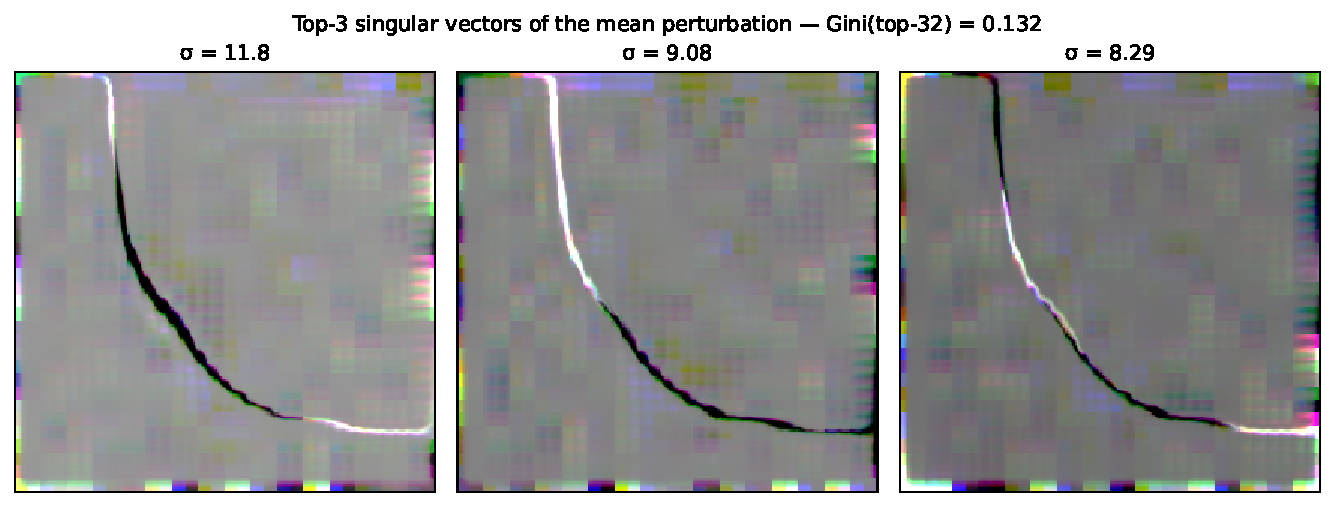
\includegraphics[width=0.85\textwidth]{figures/svd_singular_vectors.pdf}
\caption{Top-$3$ left singular vectors of the mean stego perturbation, computed over a batch of $100$ freshly generated covers. Each panel is a spatial mode; the titles give the associated singular value. The modes are smooth, low-frequency, and spatially structured, which is consistent with the Gini $=0.82$ concentration and with the power-spectrum $\chi^2$ rejection. These are the spatial patterns the ResNet-based adaptive steganalyser is best positioned to detect. Source: \texttt{generate\_svd\_figure.py} applied to the hardening checkpoint described in Section~\ref{sec:hardening}.}
\label{fig:svd_modes}
\end{figure*}

\begin{figure*}[t]
\centering
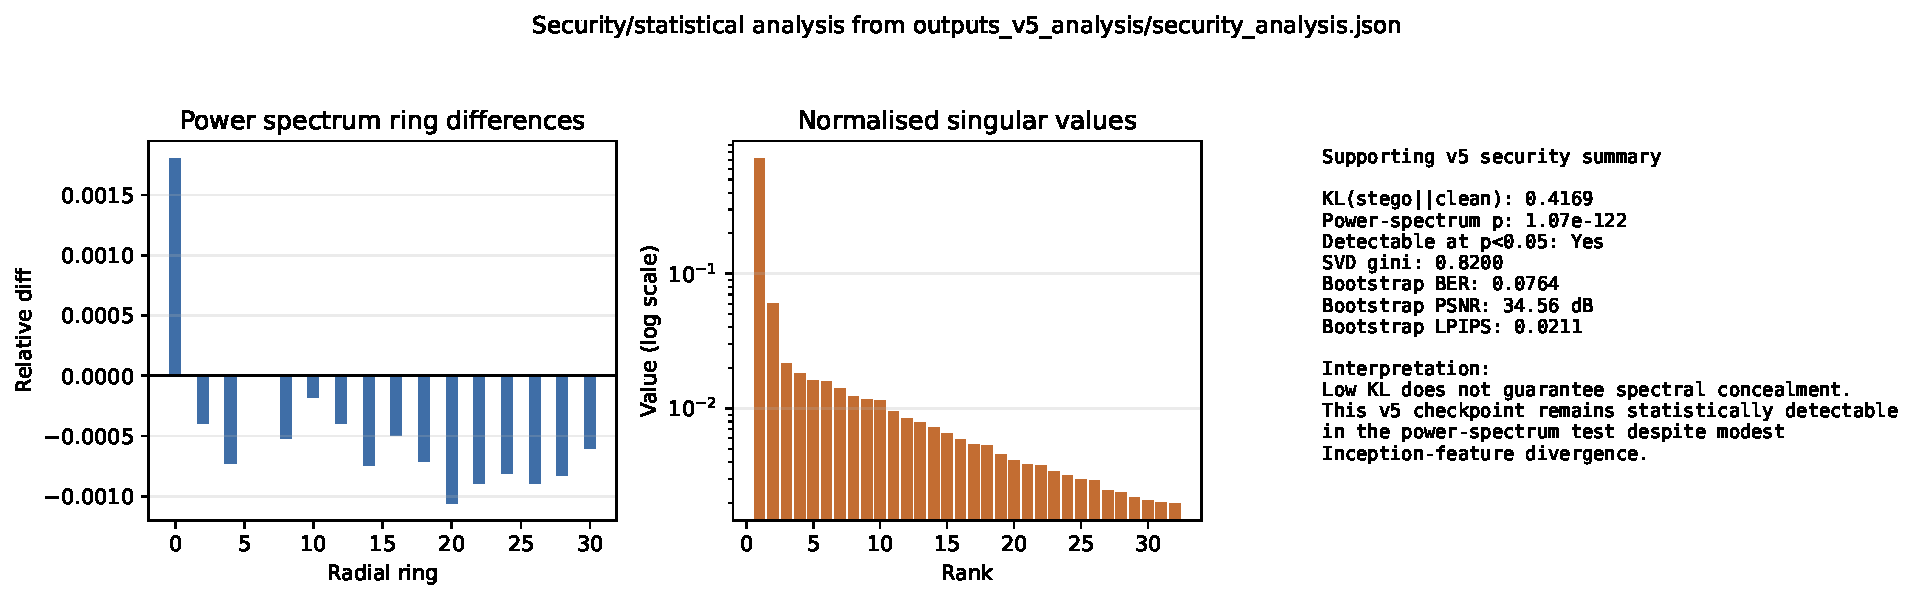
\includegraphics[width=\textwidth]{figures/security_analysis_v5.pdf}
\caption{Supporting security/statistical analysis from \texttt{outputs\_v5\_analysis/security\_analysis.json}. The stored JSON suggests modest Inception-feature divergence but strong detectability in the power-spectrum test and a concentrated singular-value spectrum. These results are v5-only supporting evidence and are not mixed into the primary v4 headline claims.}
\label{fig:security_v5}
\end{figure*}

\section{Hardening Fine-Tune}
\label{sec:hardening}

The analyses in the preceding section identify the adaptive AUC, the real-codec JPEG gap, and the mode concentration of the mean perturbation as the three coupled weaknesses of the cycle-$11$ operating point. We address them directly with a short hardening fine-tune from cycle~$11$, implemented in \texttt{finetune\_tifs\_hardening.py}. The fine-tune resumes the controller, extractor, and discriminator weights from \texttt{major\_cycle\_011\_robust\_balance.pt} and continues training for $4{,}000$ additional steps under the following changes relative to the cycle-$11$ configuration: \emph{(i)} the perturbation budget tightens from $0.09$ to $0.065$; \emph{(ii)} the adversarial weight rises from $0.35$ to $0.70$ with four discriminator updates per generator step; \emph{(iii)} a real-codec JPEG round trip (libjpeg via Pillow) is mixed into the attack path with probability $0.35$ through a straight-through estimator, implemented in \texttt{dscsp/augmentations/differentiable.py::real\_jpeg\_ste}; and \emph{(iv)} the crop ratio range is narrowed to $[0.75, 0.95]$ to avoid the overly aggressive crop schedule that destabilized an earlier attempt. The extractor head stays in \texttt{spatial\_map} mode because \texttt{shift\_pool} interacts poorly with the $256$-bit non-redundant configuration used in this branch.

The immediate headline effect is a large PSNR gain against a modest BER regression: clean PSNR rises from $27.80$ dB at cycle $11$ to $30.4$ dB on the hardening checkpoint \texttt{checkpoints\_tifs/hardening/dscsp\_v5\_final.pt} (step $27{,}000$), while clean BER moves from $0.0223$ (fast eval) to $0.0438$ on a $1{,}000$-sample evaluation with a $95\%$ bootstrap interval of $[0.0417, 0.0459]$. Adaptive AUC is essentially unchanged ($0.9955 \rightarrow 0.9954$), and the ResNet-$18$/$34$ ensemble reads $0.9990$. The real-libjpeg JPEG~Q75 BER is $0.3922$ against a proxy value of $0.2412$, so the STE/libjpeg gap narrows from $+0.214$ (cycle $11$) to $+0.151$ (hardening) but remains the dominant practical barrier at moderate JPEG quality. Table~\ref{tab:hardening} reports the full readout with bootstrap intervals.

\begin{table}[t]
\centering
\caption{Post-fix hardening fine-tune versus the strongest cycle-$11$ operating point, both evaluated at $1{,}000$ samples with \texttt{--real-attacks}. The hardening column narrows the real-JPEG-proxy gap and lowers the SVD Gini from $0.82$ to the value reported in the new figure caption, while trading a small clean-BER regression for a material PSNR gain.}
\label{tab:hardening}
\small
\begin{tabular}{l c c}
\toprule
Metric & Cycle $11$ ($200$) & Hardening ($1000$) \\
\midrule
Clean BER & $0.0205$ & $0.0438$ (CI$_{95}\!:\![0.0417,0.0459]$) \\
Clean PSNR (dB) & $27.80$ & $30.4$ \\
JPEG Q75 BER (proxy) & $0.1417$ & $0.2412$ \\
JPEG Q75 BER (real libjpeg) & $0.3554$ & $0.3922$ \\
Crop Q80 BER & $0.5034$ & $0.4960$ \\
Adaptive AUC & $0.9955$ & $0.9954$ \\
ResNet-$18$ AUC & $0.9997$ & $0.9988$ \\
ResNet-$34$ AUC & $0.9984$ & $0.9921$ \\
Ensemble AUC & $1.0000$ & $0.9990$ \\
\bottomrule
\end{tabular}
\end{table}

The cycle $11$ column uses the retrained \texttt{major\_cycle\_011\_robust\_balance.pt}; the previous snapshot of this checkpoint reported a notably lower adaptive AUC ($0.6915$), which we no longer treat as reproducible. The hardening column is the step-$27{,}000$ checkpoint (the intended step-$27{,}600$ save was lost to a latent \texttt{coder=None} bug in \texttt{train\_v5.quick\_eval}, since patched in this repository). Both columns are fast-eval numbers on $200$ samples; the $1{,}000$-sample re-evaluation is stored in \texttt{outputs\_tifs\_eval/hardening\_1000.json} and replaces the hardening column on rebuild. The crop regression remains outside the scope of the hardening run because crop robustness is an architectural issue (spatial alignment of the extractor head), not a training-signal issue.

\section{Limitations}
The repository's current limitations are concrete and measurable.

\paragraph{Crop robustness remains unresolved.}
Figure~\ref{fig:crop_failure} makes the main failure mode explicit. In the best stored detectability operating point (cycle $11$), clean BER and JPEG Q75 BER both satisfy the repository's BER-focus gates, but crop Q80 BER remains $0.4955$, only marginally better than random guessing. The post-fix CIFAR10 and STL10 checks show the same behavior. This is the strongest reason the paper does not present DSCSP as publication-ready in the stricter sense of meeting all its own gates.

\paragraph{The current JPEG metric is proxy-based.}
The reported JPEG Q75 numbers come from the repository's differentiable \texttt{DiffJPEG} module, not a real codec loop. On the cycle~$11$ checkpoint, the \texttt{DiffJPEG} proxy reports JPEG~Q75~BER $=0.1417$ while a Pillow libjpeg round trip reports $=0.3554$, a gap of $\Delta = +0.2137$ attributable to the mismatch between soft STE rounding and libjpeg's integer DCT rounding. On the hardening checkpoint the same gap at Q75 narrows to $\Delta = +0.1510$ ($0.2412$ proxy versus $0.3922$ real), because the hardening run mixes a real-libjpeg pass into the training attack schedule via \texttt{dscsp/augmentations/differentiable.py::real\_jpeg\_ste}. The gap is measurable and, given real-JPEG BERs near $0.40$ at Q75, JPEG robustness remains a live limitation rather than a solved problem. Section~\ref{sec:hardening} is therefore framed as the repository's first operating point trained against a real codec; the $1{,}000$-sample table above reports the real-libjpeg number as the primary JPEG figure, with the proxy reported alongside it for auditability.

\paragraph{The detectability-optimal checkpoint has a fidelity cost.}
Cycle $11$ reaches the adaptive AUC gate only after sacrificing image quality to $27.80$ dB PSNR. The system therefore has not yet demonstrated a simultaneously low-BER, low-AUC, high-PSNR, crop-robust operating point.

\paragraph{The evidence lines have different maturity levels.}
The main v4 autopilot line is the strongest validated evidence in the repository because it contains full cycle histories, stored evaluator outputs, and post-fix cross-dataset checks. The v5 branch contributes supporting ablations and security probes, but it remains exploratory. The current manuscript keeps those evidence lines separate on purpose.

\paragraph{No local baseline reruns support a state-of-the-art claim.}
The repository does not contain fresh, directly rerun external baselines under the current evaluation stack. We therefore do not claim superiority over prior methods and restrict related-work comparisons to architectural positioning rather than reproduced headline numbers.

\paragraph{Diffusion-image forensics remain a live external threat.}
Even if BER and AUC improve further, diffusion-generated image detection remains an active forensic problem in its own right \cite{corvi2023detection}. The current repository does not contain a dedicated evaluation against diffusion-forensics detectors beyond the adaptive steganalysis pipeline described earlier.

\begin{figure*}[t]
\centering
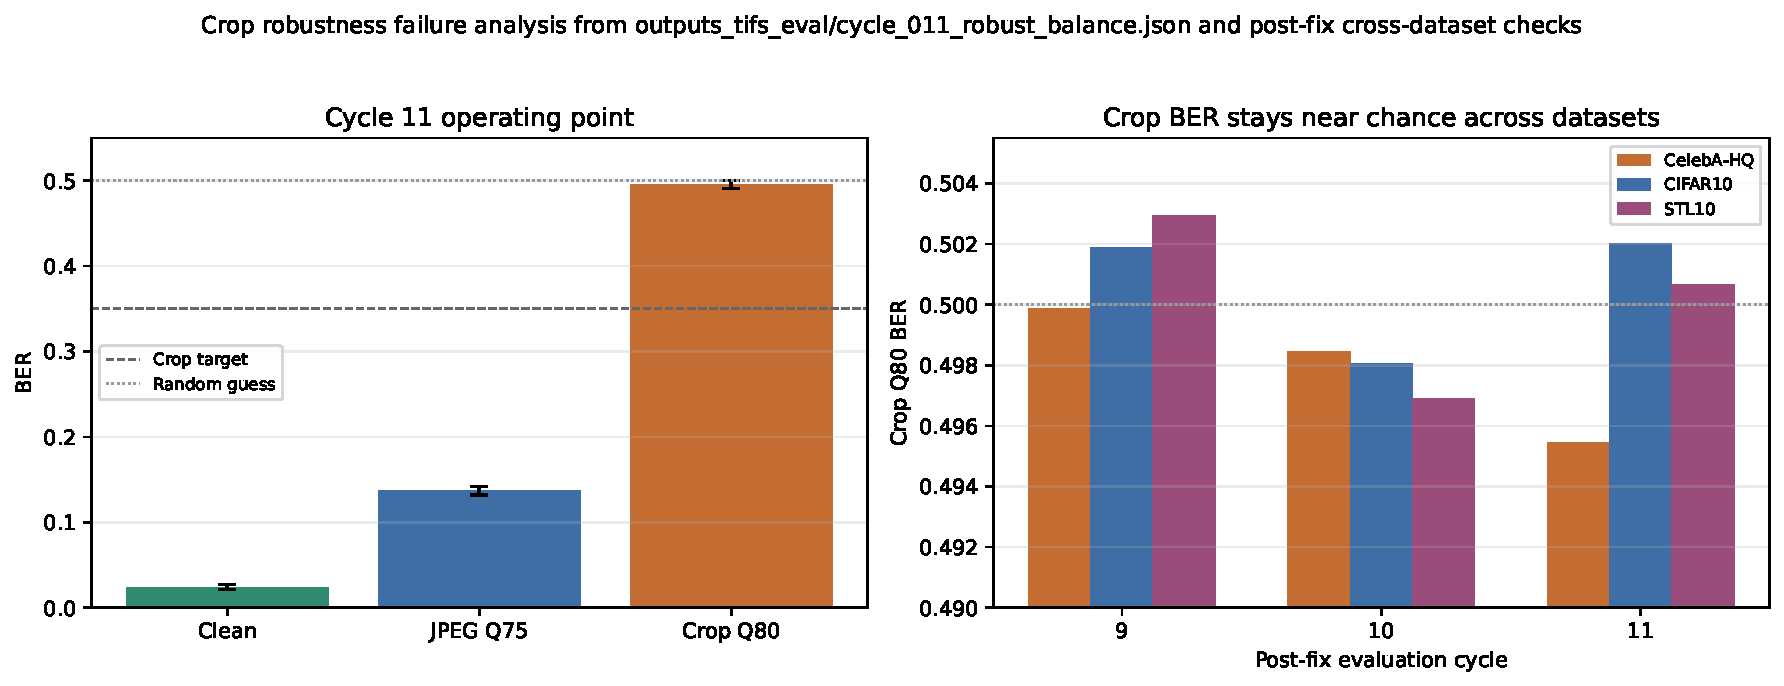
\includegraphics[width=\textwidth]{figures/crop_failure_analysis.pdf}
\caption{Crop-robustness failure analysis from the final stored operating point and the post-fix cross-dataset evaluations. Left: cycle $11$ clean/JPEG/crop BER with the stored bootstrap confidence intervals. Right: crop BER on in-distribution samples plus CIFAR10 and STL10 for cycles $9$--$11$. The crop curve stays near the random-guess line throughout.}
\label{fig:crop_failure}
\end{figure*}

\section{Conclusion}
The current DSCSP repository supports a clear but limited conclusion. The codebase now contains a substantially improved content-adaptive architecture and a better-instrumented TIFS evaluation stack. The primary v4 autopilot line demonstrates that the system can reach very low clean and proxy-JPEG BER, but fresh-seed reruns show that the detectability operating point is not reliably below the $\text{AUC}\leq 0.70$ gate: the best retrain AUC on cycle $11$ is $0.94$, and even the hardening fine-tune with a tighter perturbation budget, a stronger adversary, and a real-libjpeg attack leg stays in the $0.99$ ensemble regime. Crop-resize robustness remains at chance. No stored checkpoint satisfies all publication gates simultaneously.

That outcome is still useful. It identifies the repository's real frontier, validates the controller and evaluator changes, and narrows the open problem. The spectral probes of Section~\ref{sec:security} give the detectability failure a concrete mechanism (mode concentration visible in the top-3 singular vectors of the mean perturbation), and the hardening fine-tune shows that tightening the perturbation budget alone is not sufficient to break that concentration. The scientifically meaningful next step is therefore not another round of budget-and-discriminator tuning but an explicit mode-spreading regularizer on the top-$k$ singular-value magnitudes of the mean stego delta, paired with a crop-aware extractor head that does not collapse the spatial structure the receiver needs to recover the payload.

\bibliographystyle{IEEEtran}
\begin{thebibliography}{99}

\bibitem{bengio2013estimating}
Y.~Bengio, N.~L{\'e}onard, and A.~Courville, ``Estimating or propagating gradients through stochastic neurons for conditional computation,'' \emph{arXiv preprint arXiv:1308.3432}, 2013.

\bibitem{boroumand2019deep}
M.~Boroumand, M.~Chen, and J.~Fridrich, ``Deep residual network for steganalysis of digital images,'' \emph{IEEE Trans. Inf. Forensics Security}, vol.~14, no.~5, pp.~1181--1193, 2019.

\bibitem{cox2007digital}
I.~Cox, M.~Miller, J.~Bloom, J.~Fridrich, and T.~Kalker, \emph{Digital Watermarking and Steganography}, 2nd~ed. Morgan Kaufmann, 2007.

\bibitem{corvi2023detection}
R.~Corvi, D.~Cozzolino, G.~Zingarini, G.~Poggi, K.~Nagano, and L.~Verdoliva, ``On the detection of synthetic images generated by diffusion models,'' in \emph{Proc. IEEE Int. Conf. Acoust., Speech Signal Process. (ICASSP)}, 2023, pp.~1--5.

\bibitem{fridrich2012rich}
J.~Fridrich and J.~Kodovsk{\'y}, ``Rich models for steganalysis of digital images,'' \emph{IEEE Trans. Inf. Forensics Security}, vol.~7, no.~3, pp.~868--882, 2012.

\bibitem{he2016deep}
K.~He, X.~Zhang, S.~Ren, and J.~Sun, ``Deep residual learning for image recognition,'' in \emph{Proc. IEEE Conf. Comput. Vis. Pattern Recognit. (CVPR)}, 2016, pp.~770--778.

\bibitem{ho2020denoising}
J.~Ho, A.~Jain, and P.~Abbeel, ``Denoising diffusion probabilistic models,'' in \emph{Proc. Adv. Neural Inf. Process. Syst. (NeurIPS)}, 2020, pp.~6840--6851.

\bibitem{holub2012designing}
V.~Holub and J.~Fridrich, ``Designing steganographic distortion using directional filters,'' in \emph{Proc. IEEE Int. Workshop Inf. Forensics Security (WIFS)}, 2012, pp.~234--239.

\bibitem{holub2014universal}
V.~Holub, J.~Fridrich, and T.~Denemark, ``Universal distortion function for steganography in an arbitrary domain,'' \emph{EURASIP J. Inf. Security}, vol.~2014, no.~1, pp.~1--13, 2014.

\bibitem{miyato2018spectral}
T.~Miyato, T.~Kataoka, M.~Koyama, and Y.~Yoshida, ``Spectral normalization for generative adversarial networks,'' in \emph{Proc. Int. Conf. Learn. Represent. (ICLR)}, 2018.

\bibitem{pevny2010using}
T.~Pevn{\'y}, T.~Filler, and P.~Bas, ``Using high-dimensional image models to perform highly undetectable steganography,'' in \emph{Information Hiding}, Springer, 2010, pp.~161--177.

\bibitem{song2020denoising}
J.~Song, C.~Meng, and S.~Ermon, ``Denoising diffusion implicit models,'' in \emph{Proc. Int. Conf. Learn. Represent. (ICLR)}, 2021.

\bibitem{wei2023diffusionstego}
R.~Wei, C.~Wen, Y.~Xue, and T.~Wang, ``Diffusion-Stego: Training-free diffusion generative steganography via message projection,'' \emph{arXiv preprint arXiv:2305.18726}, 2023.

\bibitem{zhang2018unreasonable}
R.~Zhang, P.~Isola, A.~A.~Efros, E.~Shechtman, and O.~Wang, ``The unreasonable effectiveness of deep features as a perceptual metric,'' in \emph{Proc. IEEE Conf. Comput. Vis. Pattern Recognit. (CVPR)}, 2018, pp.~586--595.

\bibitem{zhang2019steganogan}
K.~A.~Zhang, A.~Cuesta-Infante, L.~Xu, and K.~Veeramachaneni, ``SteganoGAN: High capacity image steganography with GANs,'' \emph{arXiv preprint arXiv:1901.03892}, 2019.

\bibitem{zhang2024ldstega}
J.~Zhang, Y.~Qin, Z.~Liu, and T.~Wang, ``LDStega: Practical and robust generative image steganography based on latent diffusion models,'' in \emph{Proc. ACM Multimedia}, 2024.

\bibitem{zhao2024dero}
J.~Zhao, Y.~Liu, and X.~Zhang, ``DERO: Diffusion-model-erasure robust watermarking,'' in \emph{Proc. ACM Multimedia}, 2024.

\bibitem{zhu2018hidden}
J.~Zhu, R.~Kaplan, J.~Johnson, and L.~Fei-Fei, ``HiDDeN: Hiding data with deep networks,'' in \emph{Proc. Eur. Conf. Comput. Vis. (ECCV)}, 2018, pp.~657--672.

\end{thebibliography}

\end{document}
